%!TEX program = lualatex

%%%%%%%%%%%%%%
%% Run LaTeX on this file several times to get Table of Contents,
%% cross-references, and citations.

%% If you have font problems, you may edit the w-bookps.sty file
%% to customize the font names to match those on your system.

%% w-bksamp.tex. Current Version: Feb 16, 2012
%%%%%%%%%%%%%%%%%%%%%%%%%%%%%%%%%%%%%%%%%%%%%%%%%%%%%%%%%%%%%%%%
%
%  Sample file for
%  Wiley Book Style, Design No.: SD 001B, 7x10
%  Wiley Book Style, Design No.: SD 004B, 6x9
%
%
%  Prepared by Amy Hendrickson, TeXnology Inc.
%  http://www.texnology.com
%%%%%%%%%%%%%%%%%%%%%%%%%%%%%%%%%%%%%%%%%%%%%%%%%%%%%%%%%%%%%%%%

%%%%%%%%%%%%%
% 7x10
%\documentclass{wileySev}

% 6x9
\documentclass{wileySix}

%\usepackage[brazil]{babel}
%\usepackage[utf8]{inputenc}
\usepackage{polyglossia}
\usepackage{xcolor,graphicx,tikz,url}
\usepackage{listings}
\usepackage{color}
\usepackage{hyperref}
\usepackage{fontspec}
\usepackage{amsmath}
\usepackage{tikz}

\renewcommand*{\theenumi}{\thechapter.\arabic{enumi}}
\newtheorem{myDef}{Definição}

\selectlanguage{portuguese}
\renewcommand{\lstlistingname}{Listagem}
\lstdefinestyle{customc}{
  backgroundcolor=\color{yellow!20}, 
  belowcaptionskip=1\baselineskip,
  breaklines=true,
  frame=L,
  xleftmargin=\parindent,
  extendedchars=true,
  language=C++,
  showstringspaces=false,
  basicstyle=\footnotesize\ttfamily,
  keywordstyle=\bfseries\color{red!40!black},
  commentstyle=\itshape\color{green!40!black},
  otherkeywords={Ponto, QUADRADO, RETANGULO, TRIANGULO, CIRCULO, ELIPSE, CIRCUNFERENCIA, PONTO, RETA, GRAFICO},           
  emph={
  		AbreJanela,
  		PintarFundo,
  		Pintar,
  		Grafite,
  		Move,
  		Desenha,
  		Desenha1Frame,
  		MostraPlanoCartesiano,
      MudaLimitesJanela,
      CriaGrafico,
      CriaReta,
      CriaCircunferencia,
      CriaCirculo,
      CriaGrupo,
      CriaQuadrado,
      CriaTriangulo,
      CriaRetangulo,
      CriaElipse,
      CriaPonto,
      CriaPoligono,
      ApertouTecla,
      LimpaDesenho
  		},
  emphstyle={\color{blue!40!black}\bfseries},
  stringstyle=\color{orange},
  postbreak=\raisebox{0ex}[0ex][0ex]{%
  \ensuremath{\color{red}\hookrightarrow\space}},
  inputencoding=utf8,
  numbers=left,  numberstyle=\tiny
}
\lstset{escapechar=@}
\def\playAPC{\textsf{playAPC}}

%%%%%%%
%% for times math: However, this package disables bold math (!)
%% \mathbf{x} will still work, but you will not have bold math
%% in section heads or chapter titles. If you don't use math
%% in those environments, mathptmx might be a good choice.

% \usepackage{mathptmx}

% For PostScript text
\usepackage{w-bookps}

%%%%%%%%%%%%%%%%%%%%%%%%%%%%%%%%%%%%%%%%%%%%%%%%%%%%%%%%%%%%%%%%
%% Other packages you might want to use:

% for chapter bibliography made with BibTeX
% \usepackage{chapterbib}

% for multiple indices
% \usepackage{multind}

% for answers to problems
% \usepackage{answers}

%%%%%%%%%%%%%%%%%%%%%%%%%%%%%%
%% Change options here if you want:
%%
%% How many levels of section head would you like numbered?
%% 0= no section numbers, 1= section, 2= subsection, 3= subsubsection
%%==>>
\setcounter{secnumdepth}{3}

%% How many levels of section head would you like to appear in the
%% Table of Contents?
%% 0= chapter titles, 1= section titles, 2= subsection titles, 
%% 3= subsubsection titles.
%%==>>
\setcounter{tocdepth}{2}

%% Cropmarks? good for final page makeup
%% \docropmarks

%%%%%%%%%%%%%%%%%%%%%%%%%%%%%%
%
% DRAFT
%
% Uncomment to get double spacing between lines, current date and time
% printed at bottom of page.
% \draft
% (If you want to keep tables from becoming double spaced also uncomment
% this):
% \renewcommand{\arraystretch}{0.6}
%%%%%%%%%%%%%%%%%%%%%%%%%%%%%%

%%%%%%% Demo of section head containing sample macro:
%% To get a macro to expand correctly in a section head, with upper and
%% lower case math, put the definition and set the box 
%% before \begin{document}, so that when it appears in the 
%% table of contents it will also work:

\newcommand{\VT}[1]{\ensuremath{{V_{T#1}}}}

%% use a box to expand the macro before we put it into the section head:

\newbox\sectsavebox
\setbox\sectsavebox=\hbox{\boldmath\VT{xyz}}

%%%%%%%%%%%%%%%%% End Demo


\begin{document}

\booktitle{playAPC}
\subtitle{Biblioteca gráfica para programadores inexperientes}

\authors{Sinayra Pascoal Cotts Moreira\\
\affil{Universidade de Brasília}
Prof. Dr. José Carlos Loureiro Ralha\\
\affil{Universidade de Brasília}
Prof. Dr. Alexandre Zaghetto,\\
\affil{Universidade de Brasília}
}

\offprintinfo{playAPC, Primeira edição}{Sinayra P.C. Moreira}

%% Can use \\ if title, and edition are too wide, ie,
%% \offprintinfo{Survey Methodology,\\ Second Edition}{Robert M. Groves}

%%%%%%%%%%%%%%%%%%%%%%%%%%%%%%
%% 
\halftitlepage

\titlepage


\begin{copyrightpage}{2007}
Survey Methodology / Robert M. Groves . . . [et al.].
\       p. cm.---(Wiley series in survey methodology)
\    ``Wiley-Interscience."
\    Includes bibliographical references and index.
\    ISBN 0-471-48348-6 (pbk.)
\    1. Surveys---Methodology.  2. Social 
\  sciences---Research---Statistical methods.  I. Groves, Robert M.  II. %
Series.\\

HA31.2.S873 2007
001.4'33---dc22                                             2004044064
\end{copyrightpage}



\dedication{À todos os alunos que queiram fazer trabalhos bonitinhos na primeira matéria de computação da UnB}

\begin{contributors}

%\name{Prof. Dr. José Carlos Loureiro Ralha,} Departamento de Ciência da Computação - UnB, Brasília, DF, Brasil
%\name{Prof. Dr. Alexandre Zaghetto,} Departamento de Ciência da Computação - UnB, Brasília, DF, Brasil


\end{contributors}

\contentsinbrief
\tableofcontents
\listoffigures
\listoftables


% \begin{foreword}
% This is the foreword to the book.
% \end{foreword}

\begin{preface}
This is an example preface.
This is an example preface.
This is an example preface.
This is an example preface.

\prefaceauthor{R. K. Watts}
\where{Durham, North Carolina\\
September, 2007}

\end{preface}


\begin{acknowledgments}
From Dr.~Jay Young, consultant from Silver Spring, Maryland, I received
the initial push to even consider writing this book. Jay was a constant
``peer reader'' and very welcome advisor durying this year-long process.


To all these wonderful people I owe a deep sense of gratitude especially now
that this project has been completed.
\authorinitials{G. T. S.}
\end{acknowledgments}

\begin{acronyms}
\acro{UnB}{Universidade de Brasília}
\acro{APC}{Análise e Programação de Algoritmos}
\end{acronyms}

\begin{glossary}
\term{NormGibbs}Draw a sample from a posterior distribution
of data with an unknown mean and variance using Gibbs sampling.

\term{pNull}Test a one sided hypothesis from a numberically
specified posterior CDF or from a sample from the posterior

\term{sintegral}A numerical integration using Simpson's rule
\end{glossary}

\begin{symbols}
\term{A}Amplitude

\term{\hbox{\&}}Propositional logic symbol 

\term{a}Filter Coefficient

\bigskip

\term{\mathcal{B}}Number of Beats
\end{symbols}

\begin{introduction}

%% optional, but if you want to list author:

\introauthor{Sinayra Pascoal Cotts Moreira.}
{Departamento de Ciência da Computação - UnB\\
Brasília, DF, Brasil}

O índice de reprovação nas matérias iniciais do curso de Ciência da Computação da UnB tem crescido a cada semestre, bem como o índice de evasão. Apesar das tentativas de criar mais horários de plantão de dúvidas e maior disponibilidade dos monitores para essas disciplinas, o desinteresse se mantém. Visando aumentar o interesse dos alunos pelo curso, está sendo desenvolvida uma biblioteca gráfica 2D simplificada denominada playAPC.
Para o discente, a playAPC deve ser usada para consolidar os conceitos aprendidos em Análise e Programação de Algoritmos (APC) através de modelagem gráfica. Dessa forma, os alunos podem interagir com outras disciplinas do curso de modo lúdico. 

A playAPC foi desenvolvida utilizando a linguagem C++, a API OpenGL e a biblioteca GLFW 2.7. A API OpenGL deve ser suportada pela placa de vídeo presente no computador, sendo exigido a versão 1.3 no mínimo. O tutorial para instalação tanto da GLFW quanto da própria playAPC está disponível em detalhes no site Guia de Referência da playAPC \footnote{\url{http://pt-br.playcb.wikia.com/wiki/Categoria:Instala\%C3\%A7\%C3\%A3o}}. Apesar da playAPC ter sido desenvolvida em C++, o seu uso é focado primariamente para alunos que estejam a programar em C, ou seja, não é necessário conhecimento de C++ para utilizar a biblioteca, apenas utilizar a \emph{toolchain} do \emph{g++} para compilar.

Neste livro, será disponibilizado uma série de exercícios usando da playAPC focando auxiliar os professores da Univerdade de Brasília (UnB) a desenvolverem novas práticas de laboratórios das turmas de APC.

\begin{chapreferences}{1}

\bibitem{sb6}
{\em OpenGL SuperBible}.
\newblock Pearson Education Inc, 6 edition, 2014.

\bibitem{glfw}
Marcus Geelnard and Camilla Berglund.
\newblock {\em GLFW - Reference guide}, 2010.
\newblock API version 2.7.

\bibitem{cbook}
Brian~W. Kernighan and Dennis~M. Ritchie.
\newblock {\em The C Programming Language}.
\newblock 1989.

\bibitem{cppbook}
Stanley~B. Lippman, Josés Lajoile, and Barbara Moo.
\newblock {\em C++ Primer}.
\newblock 2013.
\end{chapreferences}
\end{introduction}


\part[Algoritmos sequenciais, condicionais e com repetições]
{Algoritmos sequenciais, condicionais e com repetições}


\chapter[Algoritmos sequenciais]
{Algoritmos sequenciais}


\section*{Resumo}

Estrutura sequencial é um conjunto de instruções que serão executadas em sequência. A sequência de cada instrução deve ser seguida apara a realização de uma tarefa.


%\begin{chapreferences}{1.}
%\bibliography{playAPC{}}
%\bibliographystyle{plain}
%\nocite{cbook}
%\nocite{sb6}
%\nocite{glfw}
%\nocite{cppbook}

%\end{chapreferences}

% \begin{chapreferences}{1}

% \bibitem{sb6}
% {\em OpenGL SuperBible}.
% \newblock Pearson Education Inc, 6 edition, 2014.

% \bibitem{glfw}
% Marcus Geelnard and Camilla Berglund.
% \newblock {\em GLFW - Reference guide}, 2010.
% \newblock API version 2.7.

% \bibitem{cbook}
% Brian~W. Kernighan and Dennis~M. Ritchie.
% \newblock {\em The C Programming Language}.
% \newblock 1989.

% \bibitem{cppbook}
% Stanley~B. Lippman, Josés Lajoile, and Barbara Moo.
% \newblock {\em C++ Primer}.
% \newblock 2013.
% \end{chapreferences}

\section*{Problemas}
\begin{enumerate}
\item
  Exiba um plano cartesiano de -100 a 100 com espaçamento de 5 unidades.
  \label{ex:cap01_ex1}

\item
  Desenhe um boneco palito que utilize pelo menos uma vez as seguintes geometrias:
  \begin{itemize}
  \item
    Círculo
  \item
    Elipse
  \item
    Retângulo
  \item
    Triângulo
  \item
    Quadrado
  \end{itemize}
  \label{ex:cap01_ex2}

\item
  Exiba a estrela de Davi.
  \label{ex:cap01_ex3}

\end{enumerate}


\section*{Soluções}

\subsection*{Exercício \ref{ex:cap01_ex1}}
\begin{figure}[ht]
  \centerline{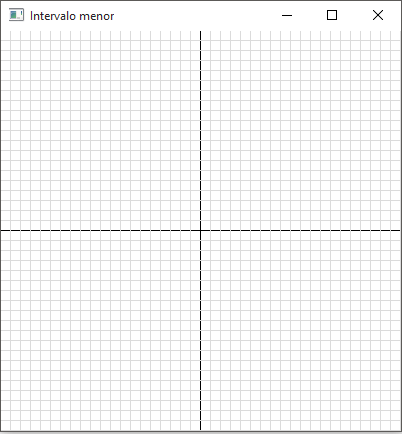
\includegraphics[width=.5\textwidth]{img/cap1_ex1.png}}
  \caption{Plano Cartesiano de -100 à 100}
  \label{fig:cap01_ex1}
\end{figure}

Esta prática se refere a exibir um Plano Cartesiano na tela com espaçamento de 5 em 5 unidades, tanto no eixo x quanto no eixo y. Com ela, o aluno poderá notar a importância da ordem de chamada de funções da \playAPC{} e a necessidade das funções \emph{AbreJanela} e \emph{Desenha}, além de verificar, com um exemplo simples, se a playAPC{} foi corretamente bem instalada.

\lstinputlisting[caption=Código fonte de Plano Cartesiano, style=customc, label=lst:cap1_ex1]{src/ex1_PrimeiraJanela.cpp}

\begin{lstlisting}[label={func:AbreJanela},language=C++]
void AbreJanela(float largura, float altura, const char* titulo)
\end{lstlisting}

A função \emph{AbreJanela}, na linha \ref{line:AbreJanela}, inicializa todas as variáveis utilizadas pela biblioteca, e preferencialmente é a chamada antes de qualquer outra função da \playAPC{}. Por padrão, o plano de renderização está limitado de (-100,100) em coordenadas $x,y$ do plano cartesiano. Este valor pode ser alterado utilizando a função \emph{MostraPlanoCartesiano} antes de chamar \emph{AbreJanela}.
Seu primeiro argumento se refere a largura da janela, o segundo a altura, sendo ambos do tipo inteiro, e o terceiro se refere ao nome que a janela terá, sendo uma string.


\begin{lstlisting}[label={func:PintarFundo},language=C++]
void PintaFundo(int red, int green, int blue)
\end{lstlisting}
A função \emph{PintarFundo}, na linha \ref{line:PintarFundo}, é específica para pintar o fundo da janela de contexto aberto pela função \emph{AbreJanela}. Seu argumentos utiliza o sistema de cores \emph{RGB} (\emph{red}, \emph{green}, \emph{blue}), utilizando a escala de 0 até 255.

\begin{lstlisting}[label={func:MostraPlanoCartesiano},language=C++]
void MostraPlanoCartesiano(int intervalo)
\end{lstlisting}
A função \emph{MostraPlanoCartesiano}, na linha \ref{line:MostraPlanoCartesiano} exibe o plano de coodernadas cartesianas, plano utilizado para o posicionamento das geometrias criadas pela \playAPC{}. Como as unidades no plano cartesiano não se referem ao posicionamento direto do pixel, a exibição do plano cartesiano com esta função serve de auxílio para o usuário posicionar suas geometrias na janela sem se preocupar com redimensionamento ou posição que a janela se encontra na tela do usuário. Para $x = 0$ e $y = 0$, as retas são pretas e as demais são cinza.
Seu único argumento se refere de quantas em quantas unidades do plano terão uma reta vertical e horizontal da cor cinza.

\begin{lstlisting}[label={func:Desenha},language=C++]
void Desenha()
\end{lstlisting}
A função \emph{Desenha}, na linha \ref{line:Desenha}, realiza o loop de renderização. Todas as geometrias criadas até esta chamada de função serão renderizadas e permanecerão estáticas, não havendo a possibilidade de posteriores animações.
Para encerrar o loop de renderização, basta fechar a janela clicando no botão de fechar ou apertando a tela \emph{ESC}. Após fechar a janela, todo o contexto da \playAPC{} será encerrado e as áreas de memórias alocadas serão liberadas.

\subsection*{Exercício \ref{ex:cap01_ex2}}
\begin{figure}[ht]
  \centerline{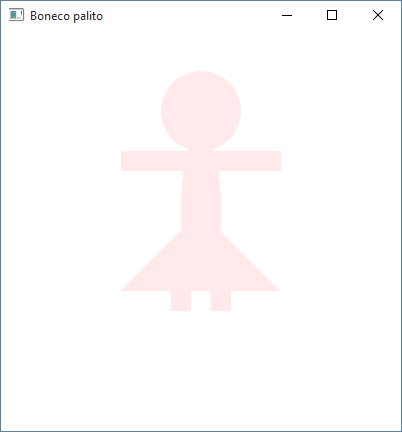
\includegraphics[width=.5\textwidth]{img/cap1_ex3.png}}
  \caption{Boneco Palito}
  \label{fig:cap01_ex2}
\end{figure}
Esta prática se refere a exibir um boneco palito e praticar a grande maioria das geometrias pré-definidas existentes na \playAPC{}. Os argumentos de cada função podem ser consultados no Guia de Referência da playAPC{} \footnote{\url{http://pt-br.playAPC{}.wikia.com/wiki/Categoria:Geometrias}}
\lstinputlisting[caption=Código fonte do boneco palito, style=customc, label=lst:cap1_ex2]{src/ex3_boneco.cpp}

\begin{lstlisting}[label={func:Ponto},language=C++]
struct Ponto{
    float x;
    float y;
}
\end{lstlisting}
Ponto, na linha \ref{line:estruturaPonto}, é uma estrutura do tipo float com dois membros, \emph{x} e \emph{y}, os quais devem ser utilizados como coordenadas do plano cartesiano 2D. Esta estrutura possui sobrecarga para os seguintes operadores =, +, -, +=, -=, == e !=.
\begin{itemize}
  \item =
    \begin{lstlisting}[style=customc,language=C++]
    Ponto p1, p2;
    (...)

    p1 = p2;
    \end{lstlisting}
   \item + (ou -)
    \begin{lstlisting}[style=customc,language=C++]
    Ponto p1, p2, p3;
    (...)

    p1 = p2 + p3;
    \end{lstlisting} 
     \item += (ou -=)
    \begin{lstlisting}[style=customc,language=C++]
    Ponto p1, p2;
    (...)

    p1 += p2;
    \end{lstlisting}

     \item == (ou !=)
    \begin{lstlisting}[style=customc,language=C++]
    Ponto p1, p2;
    (...)

    if(p1 == p2){
      (...)
    }
    \end{lstlisting}
\end{itemize}

\begin{lstlisting}[label={func:Pintarm1},language=C++]
void Pintar(int red, int green, int blue); 
void Pintar(int red, int green, int blue, geometrias_validas nome, int index);
\end{lstlisting}
A função \emph{Pintar}, na linha \ref{line:Pintarm1} pode ser utilizada de duas formas. No caso da Listagem \ref{lst:cap1_ex2}, a última geometria criada receberá a cor definida por esta função, utilizando o sistema de cores RGB. A segunda forma de utilizar esta função está ilustrada na Listagem \ref{lst:cap2_ex2}.

\begin{lstlisting}[label={func:CriaCirculo},language=C++]
int CriaCirculo(float raio, Ponto meio)
\end{lstlisting}
A função \emph{CriaCirculo}, na linha \ref{line:CriaCirculo}, cria uma geometria do tipo \emph{CIRCULO}, retornando um índice deste tipo de geometria. Seu primeiro argumento é o tamanho do raio e o segundo argumento é onde estará centrado o círculo.

\begin{lstlisting}[label={func:CriaElipse},language=C++]
int CriaElipse(float a, float b, Ponto meio)
\end{lstlisting}
A função \emph{CriaElipse}, na linha \ref{line:CriaElipse}, cria uma geometria do tipo \emph{ELIPSE}, retornando um índice deste tipo de geometria. Seu primeiro argumento é a metade do maior eixo da elipse, o segundo é a metade do menor eixo da elipse e o terceiro argumento se refere onde a elipse estará centrada.

\begin{lstlisting}[label={func:CriaQuadrado},language=C++]
int CriaQuadrado(float lado, Ponto cantoesq)
\end{lstlisting}
A função \emph{CriaQuadrado}, na linha \ref{line:CriaQuadrado}, cria uma geometria do tipo \emph{QUADRADO}, retornando um índice deste tipo de geometria. Seu primeiro argumento é o tamanho do lado do quadrado e o segundo argumento é onde ficará localizado o ponto esquerdo inferior da geometria

\begin{lstlisting}[label={func:CriaRetangulo},language=C++]
int CriaRetangulo(float base, float altura, Ponto cantoesq)
\end{lstlisting}
A função \emph{CriaRetangulo}, na linha \ref{line:CriaRetangulo}, cria uma geometria do tipo \emph{RETANGULO}, retornando um índice deste tipo de geometria. Seu primeiro argumento é a base do retângulo, o segundo a altura não-negativa dele e o último é onde ficará localizado o ponto esquerdo inferior da geometria

\begin{lstlisting}[label={func:CriaTriangulo},language=C++]
int CriaTriangulo(float base, float altura, Ponto cantoesq)
\end{lstlisting}
A função \emph{CriaTriangulo}, na linha \ref{line:CriaTriangulo}, cria uma geometria do tipo \emph{TRIANGULO}, retornando um índice deste tipo de geometria. Seu primeiro argumento é a base do triângulo, o segundo a altura não-negativa dele e o último é onde ficará localizado o ponto esquerdo inferior da geometria

\subsection*{Exercício \ref{ex:cap01_ex3}}
\begin{figure}[ht]
  \centerline{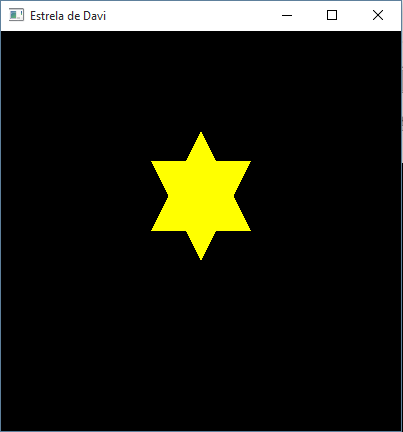
\includegraphics[width=.5\textwidth]{img/cap1_ex2.png}}
  \caption{Estrela de Davi}
  \label{fig:cap01_ex3}
\end{figure}
Esta prática se refere a exibir a estrela de Davi, feita com dois triângulos. Um triângulo foi criado com a função \emph{CriaTriangulo} e o outro com a função \emph{CriaPoligono}. Verificamos nesta prática os argumentos de \emph{CriaTriangulo} (base, altura e ponto esquerdo inferior) e, como não há como ter altura negativa, teve a necessidade de criar um polígono definido pelos três pontos \emph{p1, p2} e \emph{p3} para criar-se um triângulo \emph{de cabeça pra baixo}.
\lstinputlisting[caption=Código fonte da Estrela de Davi, style=customc, label=lst:cap1_ex3]{src/ex2_davi.cpp}

\begin{lstlisting}[label={func:CriaPoligono},language=C++]
int CriaPoligono(short int qtd, ...)
\end{lstlisting}
A função \emph{CriaPoligono}, na linha \ref{line:CriaPoligono}, cria uma geometria do tipo \emph{POLIGONO}, retornando um índice deste tipo de geometria. Seu primeiro argumento é a quantidade de pontos que serão passados para esta função, e os seguintes argumentos serão os pontos propriamente ditos. Note que a \playAPC{} é limitada no aspecto que esta função só consegue renderizar figuras convexas. Caso haja a necessidade de criação de figuras não-convexas, será necessário \emph{"quebrar"} a geometria não-convexa em duas ou mais geometrias convexas.


\chapter[Algoritmos condicionais]
{Algoritmos condicionais}



\section*{Resumo}

Estrutura condicional expõe que a instrução ou bloco de instrução só seja executada se a condição for verdadeira.


%\begin{chapreferences}{1.}
%\bibliography{playAPC{}}
%\bibliographystyle{plain}
%\nocite{cbook}
%\nocite{sb6}
%\nocite{glfw}
%\nocite{cppbook}

%\end{chapreferences}

% \begin{chapreferences}{1}

% \bibitem{sb6}
% {\em OpenGL SuperBible}.
% \newblock Pearson Education Inc, 6 edition, 2014.

% \bibitem{glfw}
% Marcus Geelnard and Camilla Berglund.
% \newblock {\em GLFW - Reference guide}, 2010.
% \newblock API version 2.7.

% \bibitem{cbook}
% Brian~W. Kernighan and Dennis~M. Ritchie.
% \newblock {\em The C Programming Language}.
% \newblock 1989.

% \bibitem{cppbook}
% Stanley~B. Lippman, Josés Lajoile, and Barbara Moo.
% \newblock {\em C++ Primer}.
% \newblock 2013.
% \end{chapreferences}

\section*{Problemas}
\begin{enumerate}
\item
  Escreva um programa que receba do usuário um valor de ângulo em graus, converta para radianos, exiba uma reta com comprimento de 50 unidades e pinte-a de acordo com as seguintes regras:
    \begin{itemize}
    \item
    Se a reta pertencer ao \emph{primeiro} quadrante, pinte-a de vermelho
    \item
    Se a reta pertencer ao \emph{segundo} quadrante, pinte-a de verde
    \item
    Se a reta pertencer ao \emph{terceiro} quadrante, pinte-a de azul
    \item
    Se a reta pertencer ao \emph{quarto} quadrante, pinte-a de preto
    \end{itemize}.
    \label{ex:cap01_ex4}
\end{enumerate}

\section*{Soluções}

\subsection*{Exercício \ref{ex:cap01_ex4}}
\begin{figure}[ht]
  \centerline{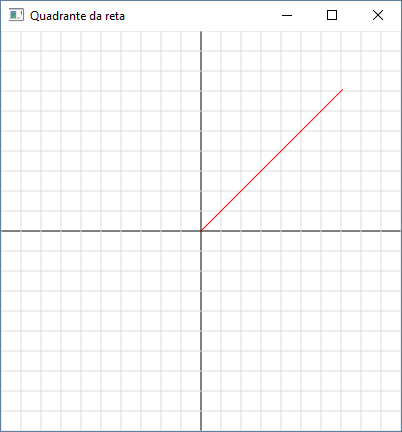
\includegraphics[width=.5\textwidth]{img/cap1_ex4.png}}
  \caption{Determinação do quadrante de uma reta baseado no ângulo de inclinação dela}
  \label{fig:cap01_ex4}
\end{figure}
Esta prática exibe uma reta com cor variada de acordo com qual quadrante ela pertence. A função \emph{Pintar} neste caso se refere a única geometria criada no programa, no caso, a reta.
\lstinputlisting[caption=Código fonte do quadrante da reta, style=customc, label=lst:cap1_ex4]{src/ex4_reta.cpp}

\begin{lstlisting}[label={func:CriaReta},language=C++]
int CriaReta(Ponto p1, Ponto p2)
\end{lstlisting}
A função \emph{CriaReta}, na linha \ref{line:CriaReta}, cria uma geometria do tipo \emph{RETA}, retornando um índice deste tipo de geometria. Seu primeiro e segundo argumento são duas variáveis do tipo Ponto.

\chapter[Algoritmos com repetição]
{Algoritmos com repetição}



\section*{Resumo}

Estruturas de repetição são criadas para que diversas instruções sejam executadas um determinado número de vezes, enquanto a condição se manter verdadeira.


%\begin{chapreferences}{1.}
%\bibliography{playAPC{}}
%\bibliographystyle{plain}
%\nocite{cbook}
%\nocite{sb6}
%\nocite{glfw}
%\nocite{cppbook}

%\end{chapreferences}

% \begin{chapreferences}{1}

% \bibitem{sb6}
% {\em OpenGL SuperBible}.
% \newblock Pearson Education Inc, 6 edition, 2014.

% \bibitem{glfw}
% Marcus Geelnard and Camilla Berglund.
% \newblock {\em GLFW - Reference guide}, 2010.
% \newblock API version 2.7.

% \bibitem{cbook}
% Brian~W. Kernighan and Dennis~M. Ritchie.
% \newblock {\em The C Programming Language}.
% \newblock 1989.

% \bibitem{cppbook}
% Stanley~B. Lippman, Josés Lajoile, and Barbara Moo.
% \newblock {\em C++ Primer}.
% \newblock 2013.
% \end{chapreferences}

\section*{Problemas}
\begin{enumerate}
\item
  Sabendo que a equação hiperbólica pode ser defina por
  $$
  \begin{matrix}
  x	& = &	a \cos(\theta) \\ 
  y	& = &	a \sin(\theta)
  \end{matrix}.
  $$
  onde $a$ é a assíntota para y e $\theta$ o ângulo equivalente ao ângulo em coordenadas polares, exiba duas espirais hiberbólicas, onde uma delas está invertida em relação a outra e coloque-as para girar.
  \label{ex:cap01_ex5}

\item
  Exiba um carrinho se movendo de $-100$ à $100$.
  \label{ex:cap01_ex6}

\item
  Construa um moinho de vento e coloque apenas as hélices para girar.
  \label{ex:cap01_ex7}
\end{enumerate}

\section*{Soluções}

\subsection*{Exercício \ref{ex:cap01_ex5}}
\begin{figure}[ht]
  \centerline{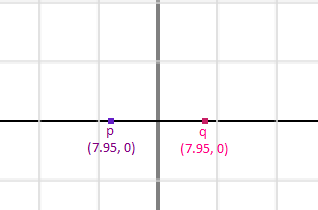
\includegraphics[width=.5\textwidth]{img/cap1_ex6.png}}
  \caption{Duas espirais hiperbólicas girando}
  \label{fig:cap01_ex5}
\end{figure}
Esta prática ilustra como a função \emph{Desenha1Frame} pode ser utilizada. Na linha \ref{line:ex6_for} até a linha \ref{line:ex6_forend}, a cada iteração são criados dois pontos, um de cada espiral.
\lstinputlisting[caption=Código fonte da galáxia expiral, style=customc, label=lst:cap1_ex5]{src/ex6_galaxy.cpp}


\begin{lstlisting}[label={func:CriaPonto},language=C++]
int CriaPonto(Ponto p)
\end{lstlisting}
A função \emph{CriaPonto}, na linha \ref{line:CriaPonto}, cria uma geometria do tipo \emph{PONTO}, retornando um índice deste tipo de geometria. Seu único argumento é uma variável do tipo Ponto. Uma geometria do tipo \emph{PONTO} é renderizada como um pixel.

\begin{lstlisting}[label={func:Grafite},language=C++]
void Grafite(int espessura)
\end{lstlisting}
A função \emph{Grafite}, na linha \ref{line:Grafite}, aumenta as linhas de rasterização da última geometria criada, variando de 1 a $\infty$. Por padrão, todas as geometrias começam com esta linha igual a 1. Esta função pode ser usada para deixar mais visível geometrias do tipo \emph{PONTO}, que possuem 1 pixel de tamanho.

\begin{lstlisting}[label={func:Desenha1Frame},language=C++]
int Desenha1Frame()
\end{lstlisting}
A função \emph{Desenha1Frame}, na linha \ref{line:Desenha1Frame}, renderiza pelo menos $\frac{1}{60}$ segundos da cena, possuindo um controle de 60 frames por segundo. Caso o usuário feche a janela ou aperte a tecla ESC, esta função retornará 0 e encerrará o processo de renderização. Caso contrário, retornará 1.

\begin{lstlisting}[label={func:Gira},language=C++]
void Gira(float theta)
void Gira(float theta, int index)
\end{lstlisting}
A função \emph{Gira}, na linha \ref{line:Giram1}, é uma das três funções de transformação implementadas na \playAPC{}. Há duas formas de utilizar esta função. No caso da Listagem \ref{lst:cap1_ex5}, seu argumento é um ângulo $\theta$ em graus e ele irá girar todas as geometrias criadas, recalculando a posição de cada pixel utilizando a Definição \ref{def:rotacao}. 

\begin{myDef} 
Seja $x$ a coordenada do eixo x original do ponto, $y$ a coordenada do eixo y original do ponto, $x'$ a coordenada resultado do eixo, $y'$ a coordenada resultante do eixo y e $\theta$ o ângulo em graus de rotação.
$$
  \begin{matrix}
  x' = x\cos \theta  - y \sin \theta &\\
  y' = x\sin \theta  + y \cos \theta
  \end{matrix}
$$
\label{def:rotacao}
\end{myDef}

\begin{lstlisting}[label={func:ApertouTecla},language=C++]
int ApertouTecla(int tecla)
\end{lstlisting}
A função \emph{ApertouTecla}, na linha \ref{line:ApertouTecla}, verifica se o usuário pressionou a tecla \emph{tecla} naquela cena. Seu único argumento pode variar de acordo com a Tabela \ref{tab:teclas}.

~\begin{table}
  \caption{Teclas reconhecidas pela \playAPC{}}
  \centering
    \begin{tabular}{lc}
    \hline
    Valor&\bf Descrição \\
    \hline
    GLFW\_KEY\_$n$  & Teclas alfanuméricas ($n \in (0..9)$ ou $n \in (A..Z)$)  \\
    GLFW\_KEY\_SPACE  & Espaço \\
    GLFW\_KEY\_ESC  & Escape \\
    GLFW\_KEY\_F$n$  & Function key ($n \in (0..25)$) \\
    GLFW\_KEY\_LEFT  & Seta para esquerda \\
    GLFW\_KEY\_UP  & Seta para cima \\
    GLFW\_KEY\_DOWN  & Seta para baixo \\
    GLFW\_KEY\_RIGHT  & Seta para direita \\
    GLFW\_KEY\_LCONTROL  & Control esquerdo \\
    GLFW\_KEY\_RCONTROL  & Control direito \\
    GLFW\_KEY\_LALT  & Alt esquerdo \\
    GLFW\_KEY\_RALT  & Alt direito \\
    GLFW\_KEY\_TAB  & Tabulador \\
    GLFW\_KEY\_ENTER  & Enter \\
    GLFW\_KEY\_BACKSPACE  & Backspace \\
    GLFW\_KEY\_INSERT  & Insert \\
    GLFW\_KEY\_DEL  & Delete \\
    GLFW\_KEY\_PAGEUP  & Page up \\
    GLFW\_KEY\_PAGEDOWN  & Page down \\
    GLFW\_KEY\_HOME  & Home \\
    GLFW\_KEY\_END  & End \\
    GLFW\_KEY\_KP\_$n$  & Teclas numéricas do keypad ($n \in (0..9)$)\\
    GLFW\_KEY\_KP\_DIVIDE  & Tecla dividir do keypad ( \div )\\
    GLFW\_KEY\_KP\_MULTIPLY  & Tecla multiplicar do keypad ( \times )\\
    GLFW\_KEY\_KP\_SUBTRACT  & Tecla subtrair do keypad ( - )\\
    GLFW\_KEY\_KP\_ADD  & Tecla adição do keypad ( + )\\
    GLFW\_KEY\_KP\_EQUAL  & Tecla igual do keypad ( = )\\
    GLFW\_KEY\_KP\_NUMLOCK  & Tecla Numlock do keypad ( = )\\
    GLFW\_KEY\_CAPS\_LOCK  & Caps lock\\
    GLFW\_KEY\_SCROLL\_LOCK  & Scroll lock\\
    GLFW\_KEY\_PAUSE  & Pause\\
    GLFW\_KEY\_MENU  & Menu\\
    \hline
  \end{tabular}
  \label{tab:teclas}
\end{table}


\subsection*{Exercício \ref{ex:cap01_ex6}}
\begin{figure}[ht]
  \centerline{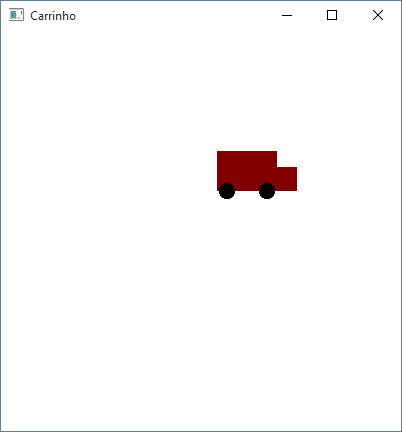
\includegraphics[width=.5\textwidth]{img/cap1_ex5.png}}
  \caption{Carro se movendo da posição -100 até a posição 100}
  \label{fig:cap01_ex6}
\end{figure}
Esta prática exibe um carro construído com dois retângulos e dois círculos, agrupados com a função \emph{CriaGrupo}, movendo-se da posição -100 até a posição 100. Nota-se que todas as geometrias que estão abaixo da função \emph{CriaGrupo} pertencem a um único grupo, o grupo \emph{carro}.
\lstinputlisting[caption=Código fonte do carro andando, style=customc, label=lst:cap1_ex6]{src/ex5_carrinho.cpp}

\begin{lstlisting}[label={func:CriaGrupo},language=C++]
int CriaGrupo()
\end{lstlisting}
A função \emph{CriaGrupo}, na linha \ref{line:CriaGrupo}, agrupará todo um conjunto de geometrias, associando todas a uma única variável, em um único conjunto. Desta forma, é possível transformar um conjunto de geometrias de forma independente, apenas referenciando a variável do grupo.

\subsection*{Exercício \ref{ex:cap01_ex7}}
\begin{figure}[ht]
  \centerline{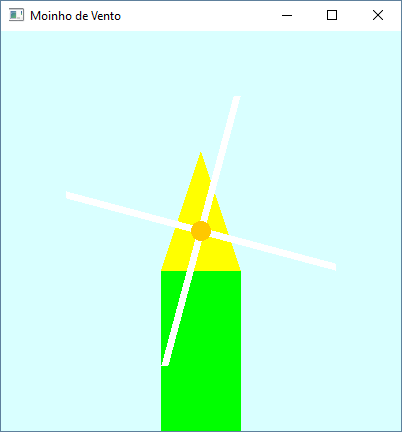
\includegraphics[width=.5\textwidth]{img/cap1_ex7.png}}
  \caption{Moinho de vento}
  \label{fig:cap01_ex7}
\end{figure}
Esta prática exibe um moinho de vento criado com um grupo composto por um triângulo e um retângulo, o grupo \emph{moinho}, e outro grupo composto pelas hélices, o grupo \emph{grupo}. Somente o \emph{grupo} sofre a ação de girar. 
\lstinputlisting[caption=Código fonte do moinho, style=customc, label=lst:cap1_ex7]{src/ex7_moinho.cpp}


\part[Estrutura de dados n-dimensionais homogêneas]
{Estrutura de dados n-dimensionais homogêneas}


\chapter[Vetores]
{Vetores}



\section{Resumo}

Vetores são um tipo de estrutura que podem armazenar um tamanho fixo de elementos do mesmo tamanho e mesmo tipo, alocados em memória contígua. Utiliza-se vetores como um tipo de lista unidimensional, acessada através de índices.


%\begin{chapreferences}{1.}
%\bibliography{playcb}
%\bibliographystyle{plain}
%\nocite{cbook}
%\nocite{sb6}
%\nocite{glfw}
%\nocite{cppbook}

%\end{chapreferences}

% \begin{chapreferences}{1}

% \bibitem{sb6}
% {\em OpenGL SuperBible}.
% \newblock Pearson Education Inc, 6 edition, 2014.

% \bibitem{glfw}
% Marcus Geelnard and Camilla Berglund.
% \newblock {\em GLFW - Reference guide}, 2010.
% \newblock API version 2.7.

% \bibitem{cbook}
% Brian~W. Kernighan and Dennis~M. Ritchie.
% \newblock {\em The C Programming Language}.
% \newblock 1989.

% \bibitem{cppbook}
% Stanley~B. Lippman, Josés Lajoile, and Barbara Moo.
% \newblock {\em C++ Primer}.
% \newblock 2013.
% \end{chapreferences}


\section{Criando um gráfico}
\begin{figure}[ht]
  \centerline{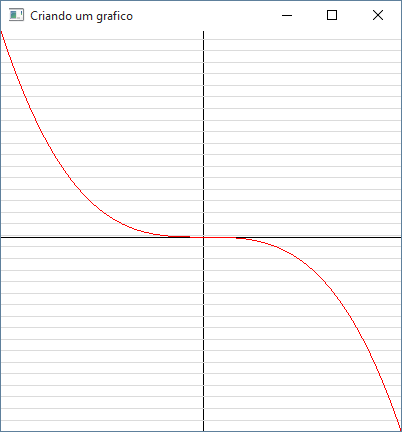
\includegraphics[width=.5\textwidth]{img/cap2_ex8.png}}
  \caption{Gráfico do polinômio $-x^3$}
  \label{fig:cap02_ex1}
\end{figure}
Esta prática mostra como construir um gráfico a partir de um vetor de Pontos. Cada posição em \emph{y} de cada ponto é calculada dentro do loop. Por padrão, os limites da janela de exibição da playCB vão de -100 à 100, entretanto, os valores em \emph{y} nesta função variam de $-125.000$ até $125.000$, tendo a necessidade de mudar o limite de exibição com a função \emph{MudaLimitesJanela(125000)}.
\lstinputlisting[caption=Código fonte de polinômio, style=customc, label=lst:cap2_ex8]{src/ex8_grafico.cpp}

\chapter[Matrizes]
{Matrizes}



\section{Resumo}

Assim como vetores, matrizes são um tipo de estrutura que armazena dados de mesmo tamanho e mesmo tipo, mas são utilizadas de maneira n-dimensional. O modo mais comum de utilizar matriz é usando-a na forma bidimensional, onde os dados são tratados como se estivessem numa tabela, com linhas e colunas.


%\begin{chapreferences}{1.}
%\bibliography{playcb}
%\bibliographystyle{plain}
%\nocite{cbook}
%\nocite{sb6}
%\nocite{glfw}
%\nocite{cppbook}

%\end{chapreferences}

% \begin{chapreferences}{1}

% \bibitem{sb6}
% {\em OpenGL SuperBible}.
% \newblock Pearson Education Inc, 6 edition, 2014.

% \bibitem{glfw}
% Marcus Geelnard and Camilla Berglund.
% \newblock {\em GLFW - Reference guide}, 2010.
% \newblock API version 2.7.

% \bibitem{cbook}
% Brian~W. Kernighan and Dennis~M. Ritchie.
% \newblock {\em The C Programming Language}.
% \newblock 1989.

% \bibitem{cppbook}
% Stanley~B. Lippman, Josés Lajoile, and Barbara Moo.
% \newblock {\em C++ Primer}.
% \newblock 2013.
% \end{chapreferences}


\section{Criando um gráfico}
\begin{figure}[ht]
  \centerline{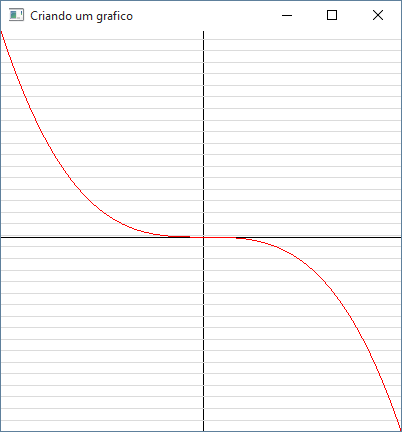
\includegraphics[width=.5\textwidth]{img/cap2_ex8.png}}
  \caption{Gráfico do polinômio $-x^3$}
  \label{fig:cap02_ex1}
\end{figure}
Esta prática mostra como construir um gráfico a partir de um vetor de Pontos. Cada posição em \emph{y} de cada ponto é calculada dentro do loop. Por padrão, os limites da janela de exibição da playCB vão de -100 à 100, entretanto, os valores em \emph{y} nesta função variam de $-125.000$ até $125.000$, tendo a necessidade de mudar o limite de exibição com a função \emph{MudaLimitesJanela(125000)}.
\lstinputlisting[caption=Código fonte de polinômio, style=customc, label=lst:cap2_ex8]{src/ex8_grafico.cpp}


\part[Subalgoritmos]
{Funções}


\chapter[Subalgoritmos]
{Funções}



\section*{Resumo}

Uma função é um conjunto de instruções que, ao final da função, executa uma tarefa. Todo programa C possui pelo menos uma função, a \emph{main}.

%\begin{chapreferences}{1.}
%\bibliography{playcb}
%\bibliographystyle{plain}
%\nocite{cbook}
%\nocite{sb6}
%\nocite{glfw}
%\nocite{cppbook}

%\end{chapreferences}

% \begin{chapreferences}{1}

% \bibitem{sb6}
% {\em OpenGL SuperBible}.
% \newblock Pearson Education Inc, 6 edition, 2014.

% \bibitem{glfw}
% Marcus Geelnard and Camilla Berglund.
% \newblock {\em GLFW - Reference guide}, 2010.
% \newblock API version 2.7.

% \bibitem{cbook}
% Brian~W. Kernighan and Dennis~M. Ritchie.
% \newblock {\em The C Programming Language}.
% \newblock 1989.

% \bibitem{cppbook}
% Stanley~B. Lippman, Josés Lajoile, and Barbara Moo.
% \newblock {\em C++ Primer}.
% \newblock 2013.
% \end{chapreferences}

\section*{Problemas}
\begin{enumerate}
\item
  Crie dois retângulos e posicione-os aleatoriamente em $x$. Coloque uma circunferência no topo do primeiro retângulo e receba do usuário dois valores: ângulo e velocidade. Dado estes valores, calcule e exiba a trajetória balística da circunferência sendo lançada para o outro retângulo. Exiba mensagem caso o usuário consiga acertar o prédio ou não e, em seguida, caso o usuário deseje jogar novamente, sorteie novamente a posição dos retângulos.

  \label{ex:cap03_ex1}
  
\item
  Crie o jogo Snake com as seguintes configurações
  \begin{itemize}
  \item
    A cabeça não pode estar na mesma posição que o corpo
  \item
    A cabeça não pode estar na mesma posição que a parede
  \end{itemize}
  \emph{SUGESTÃO: Utilize a lógica do exercício \ref{ex:cap02_ex1} }

  \label{ex:cap03_ex2}

\end{enumerate}

\section*{Soluções}

\subsection*{Exercício \ref{ex:cap03_ex1} }
\begin{figure}[ht]
  \centerline{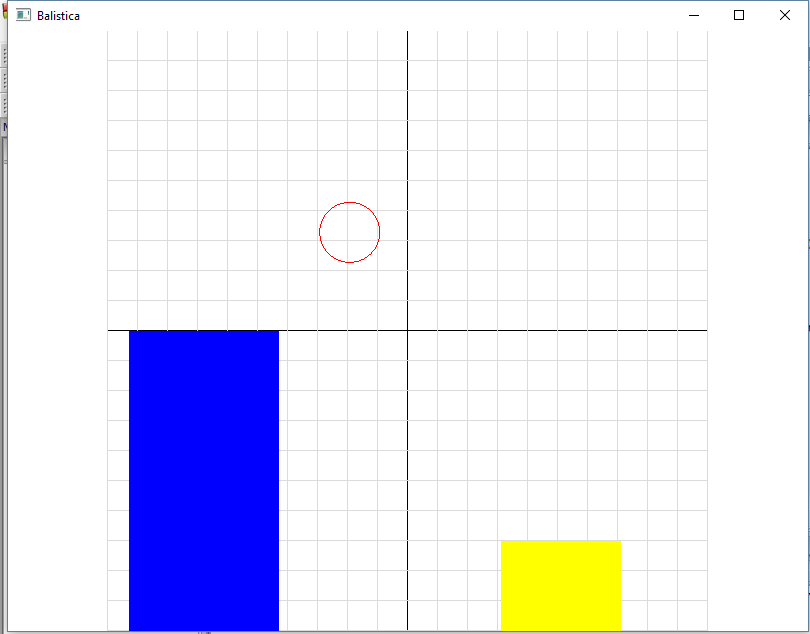
\includegraphics[width=.5\textwidth]{img/cap3_ex12.png}}
  \caption{Lançador Balístico}
  \label{fig:cap03_ex2}
\end{figure}
Esta prática ilustra como a função \emph{LimpaDesenho} é usada para poder redesenhar outras cenas.
\lstinputlisting[caption=Código fonte do lançador balístico, style=customc, label=lst:cap3_ex1]{src/ex12_balistica.cpp}

\begin{lstlisting}[label={func:LimpaDesenho},language=C++]
void LimpaDesenho() 
\end{lstlisting}
A função \emph{LimpaDesenho}, na linha \ref{line:LimpaDesenho}, destrói todas as geometrias e retorna toda a \emph{playAPC} para o estado padrão, com exceção dos limites do plano cartesiano.

\subsection*{Exercício \ref{ex:cap03_ex2} }
\begin{figure}[ht]
  \centerline{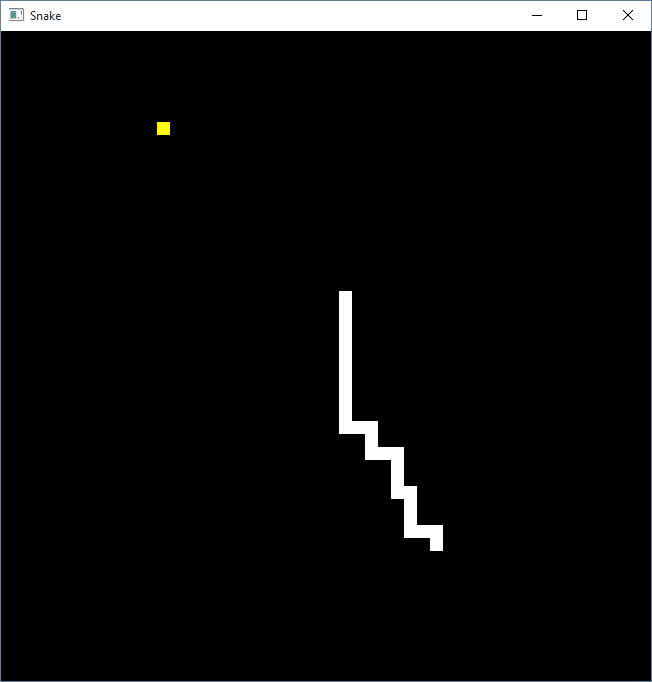
\includegraphics[width=.5\textwidth]{img/cap3_ex10.png}}
  \caption{Jogo Snake}
  \label{fig:cap03_ex2}
\end{figure}
Esta prática ilustra como a função \emph{ApertaTecla} e \emph{MudaLimitesJanela} podem ser utilizadas: a primeira para lidar com input de teclado \footnote{\url{http://pt-br.playcb.wikia.com/wiki/Aperta_Tecla}} e a segunda para ajustar o plano onde as geometrias serão desenhadas.
\lstinputlisting[caption=Código fonte de Snake, style=customc, label=lst:cap3_ex1]{src/ex10_snake.cpp}


\part[Recursão]
{Recursão}


\chapter[Recursão]
{Recursão}



\section*{Resumo}

Recursão é uma sub-rotina que pode invocar a si mesma, contendo, a cada chamada, uma pedaço menor da solução final.

%\begin{chapreferences}{1.}
%\bibliography{playcb}
%\bibliographystyle{plain}
%\nocite{cbook}
%\nocite{sb6}
%\nocite{glfw}
%\nocite{cppbook}

%\end{chapreferences}

% \begin{chapreferences}{1}

% \bibitem{sb6}
% {\em OpenGL SuperBible}.
% \newblock Pearson Education Inc, 6 edition, 2014.

% \bibitem{glfw}
% Marcus Geelnard and Camilla Berglund.
% \newblock {\em GLFW - Reference guide}, 2010.
% \newblock API version 2.7.

% \bibitem{cbook}
% Brian~W. Kernighan and Dennis~M. Ritchie.
% \newblock {\em The C Programming Language}.
% \newblock 1989.

% \bibitem{cppbook}
% Stanley~B. Lippman, Josés Lajoile, and Barbara Moo.
% \newblock {\em C++ Primer}.
% \newblock 2013.
% \end{chapreferences}

\section*{Problemas}
\begin{enumerate}
\item
  Exiba passo a passo a solução da Torre de Hanói para, no máximo, 5 discos.
  \label{ex:cap04_ex1}

\item
  Sabendo que a curva de Koch é construída que toma, como base, um segmento de reta de tamanho $n$. Na extremidade deste primeiro segmento, desenha-se outro segmento de reta de tamanho $n$, porém com uma curvatura de $60º$ em relação ao primeiro. Na extremidade deste segundo segmento, desenha-se outra curva de reta de tamanho $n$, mas agora com a curvatura de $120º$ em relação ao primeiro. Por fim, desenha-se outro segmento de reta de tamanho $n$ na extremidade do terceiro segmento.
    \begin{enumerate}
      \item Exiba a curva de Koch de ordem $n$
        \label{ex:cap04_ex2a}
      \item Exiba um floco de neve de ordem $n$ baseado na curva de Koch
        \label{ex:cap04_ex2b}
    \end{enumerate}
  \label{ex:cap04_ex2}
\item
  A curva de Sierpiński preenche todo o espaço disponível sem cortar suas próprias linhas, sendo mutuamente recursiva entre quatro funções. AQUI TEM UMA EXPLICAÇÃO DAS REGRAS DESSA CURVA. Exiba a curva de Sierpiński de ordem $n$.
  \label{ex:cap04_ex3}
\end{enumerate}

\section*{Soluções}

\subsection*{Exercício \ref{ex:cap04_ex1} }
\begin{figure}[ht]
  \centerline{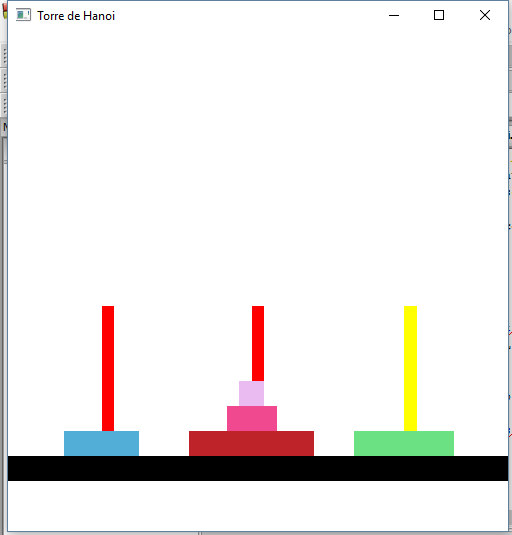
\includegraphics[width=.5\textwidth]{img/cap4_ex13.png}}
  \caption{Solucionador da torre de Hanói}
  \label{fig:cap04_ex1}
\end{figure}
Esta prática ilustra como mover cada geometria utilizando retorno da função \emph{CriaGrupo} para mover cada peça da torre de Hanoi para uma posição específica.
\lstinputlisting[caption=Código fonte da torre de Hanói, style=customc, label=lst:cap4_ex1]{src/ex13_hanoi.cpp}

\subsection*{Exercício \ref{ex:cap04_ex2} }
\subsubsection*{Item \ref{ex:cap04_ex2a}}
\begin{figure}[ht]
  \centerline{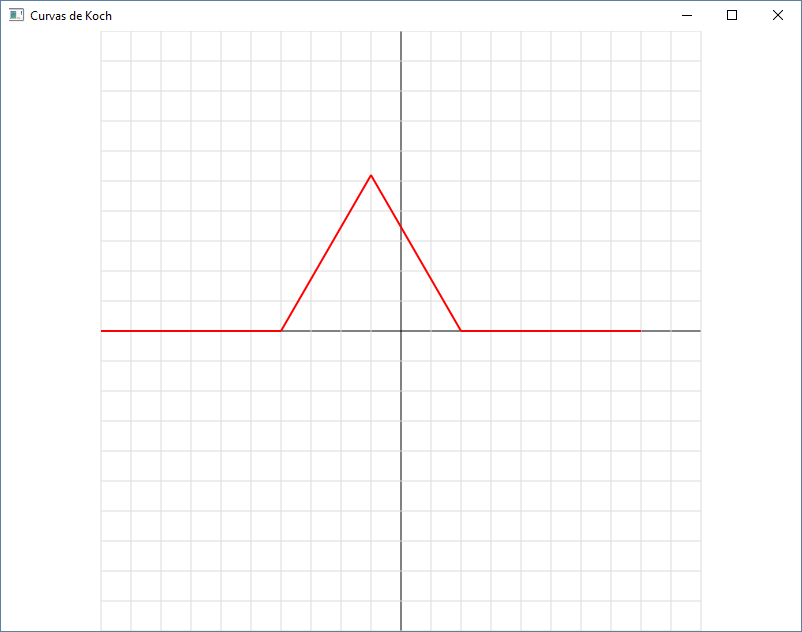
\includegraphics[width=.5\textwidth]{img/cap4_ex14.png}}
  \caption{Curva de Koch de ordem 3}
  \label{fig:cap04_ex2a}
\end{figure}
Esta prática reforça o modo de utilização da função CriaReta, usando a função \emph{movaCaneta}, na linha \ref{line:movaCaneta}.
\lstinputlisting[caption=Código fonte da curva de koch, style=customc, label=lst:cap4_ex1]{src/ex14_koch.cpp}

\subsubsection*{Item \ref{ex:cap04_ex2b}}
\begin{figure}[ht]
  \centerline{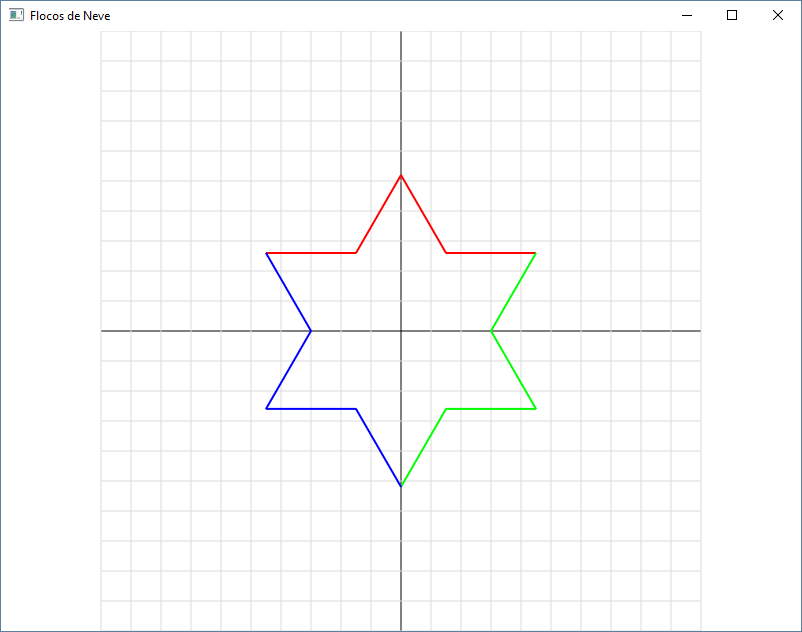
\includegraphics[width=.5\textwidth]{img/cap4_ex15.png}}
  \caption{Floco de neve}
  \label{fig:cap04_ex2b}
\end{figure}
\lstinputlisting[caption=Código fonte do floco de neve, style=customc, label=lst:cap4_ex1]{src/ex15_snowflake.cpp}


\subsection*{Exercício \ref{ex:cap04_ex3} }
\begin{figure}[ht]
  \centerline{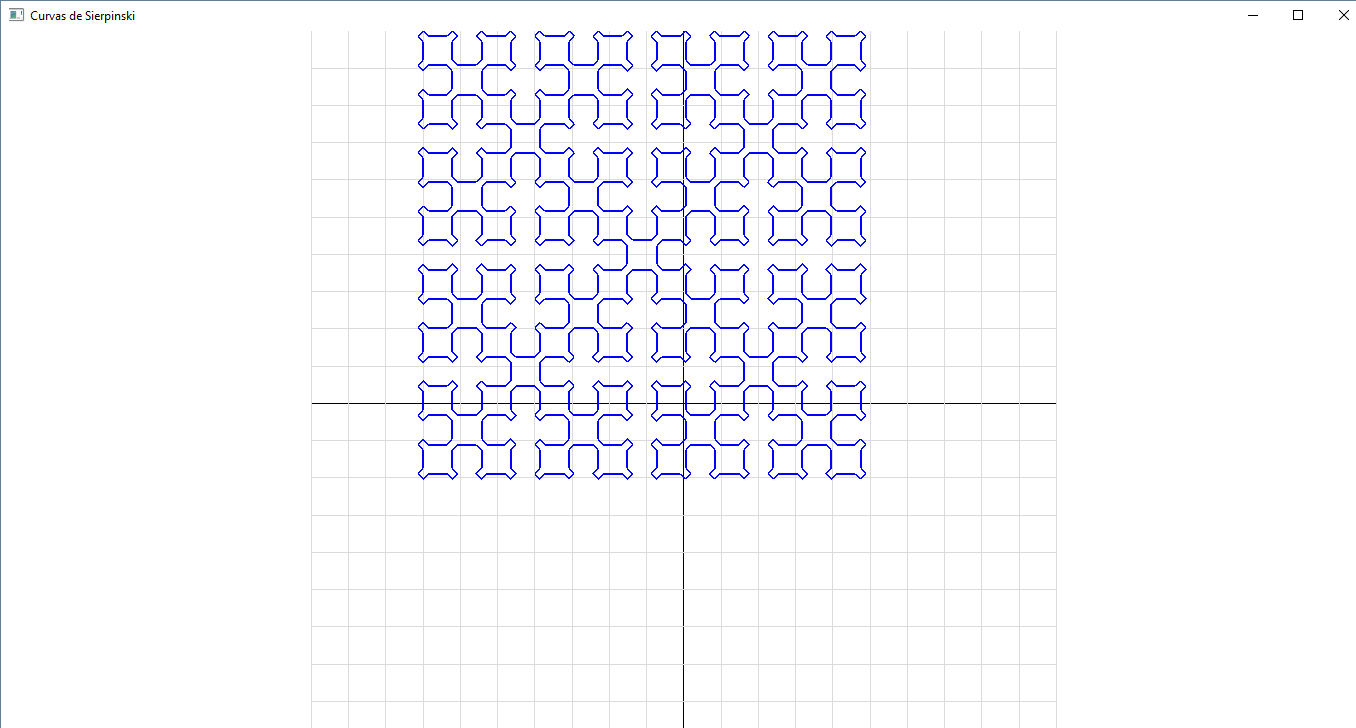
\includegraphics[width=.5\textwidth]{img/cap4_ex16.png}}
  \caption{Curva de Sierpiński}
  \label{fig:cap04_ex3}
\end{figure}
Esta prática reforça o modo de utilizar a função \emph{CriaReta}, usando as implementações das funções das linhas \ref{line:pontoA}, \ref{line:pontoB}, \ref{line:pontoC} e \ref{line:pontoD}.
\lstinputlisting[caption=Curva de Sierpiński, style=customc, label=lst:cap4_ex1]{src/ex16_sierpinski.cpp}

\part[Exercícios extras]
{Exercícios extras}


\chapter[Exercícios extras]
{Exercícios extras}



\section*{Resumo}

Este capítulo reúne uma bateria de exercícios envolvendo todos os capítulos abordados durante o livro.

\section*{Problemas}
\begin{enumerate}
\item
  A partir de um ponto no mapa, simule um geiser inundando o terreno montanhoso com água. Considere que:
  \begin{itemize}
  	\item O terreno é construído randomicamente, onde sua altura varia entre 0 à 255.
  	\item Se valor da altura igual a 0, o terreno é verde puro. Se for maior que 0, ele varia sua coloração de vermelho de modo que, ao atingir valor de altura 255, sua cor seja amarelo puro.
  	\item A cada iteração, o valor de água sobe 10 unidades e espalha-se igualmente entre o terreno.
  \end{itemize}
  \label{ex:cap05_ex1}

  \begin{figure}[H]
    \centerline{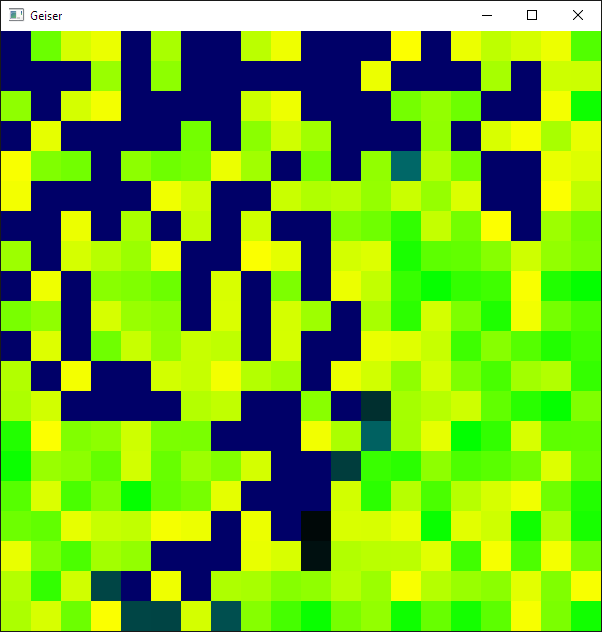
\includegraphics[width=.5\textwidth]{img/cap5_ex18.png}}
    \caption{Simulador de inundação}
    \label{fig:cap04_ex1}
  \end{figure}

\item
	Faça uma animação onde a lua está em órbita espiral em direção à terra. Ao atingir a terra, esta é jogada para fora da tela.
\label{ex:cap05_ex2}

  \begin{figure}[ht]
    \centerline{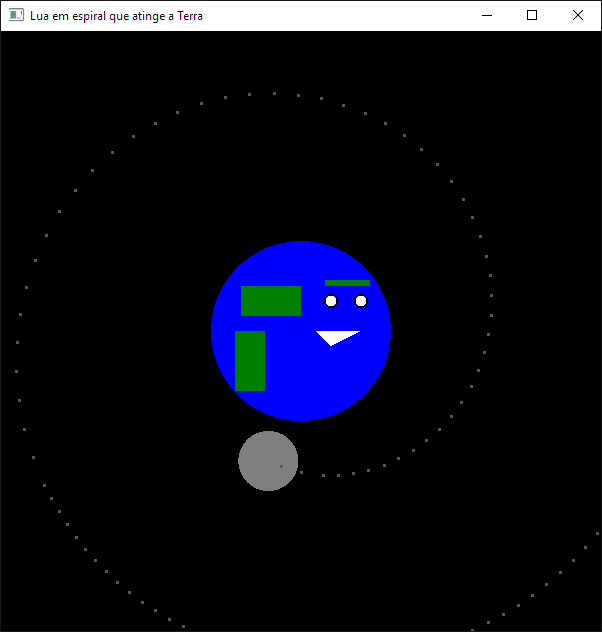
\includegraphics[width=.5\textwidth]{img/cap5_ex19.png}}
    \caption{Lua em órbita espiral}
    \label{fig:cap04_ex1}
  \end{figure}

\item
	Faça uma animação onde simule o funcionamento de um sonar, com os seguintes aspectos:
	\begin{itemize}
  	\item Há três seres na cena: um alienígena, um caça e um ruído.
  	\item O ruído realiza uma trajetória de um 8 deitado, $\infty$. Quando o ruído se aproxima do centro $(0,0)$ do sonar, ele desaparece, reaparecendo na tela depois de um certo tempo.
  	\item O caça realiza trajetória descrito pela Equação \ref{eq:cap05_ex3_1}.
  	\begin{equation}\label{eq:cap05_ex3_1}
  	\left\{\begin{matrix}
	 50 \cos(\alpha)\sqrt{2\cos(2\alpha)} & = x \\ 
	 50 \sin(\alpha)\sqrt{2\cos(2\alpha)} & = y
	\end{matrix}\right.
  	\end{equation}
  	Onde $\alpha$ é incrementado durante o loop.
  	\item O alienígena começa seu movimento, $dir$ indo da esquerda para direita. Enquanto $\alpha$ é incrementado a cada iteração do loop, há um $\theta$ que irá variar entre $0$ e $4\pi$. Toda vez que $\theta$ atingir $4\pi$, $\theta$ começa a variar de $0$ e $4\pi$ novamente, invertendo a direção $dir$ do alienígena.
  	Sendo assim, a trajetória do alienígena é descrita pela Equação \ref{eq:cap05_ex3_2}.
  	
  	\begin{equation}\label{eq:cap05_ex3_2}
  	\left\{\begin{matrix}
	 200 \cos(\theta \times dir)\div \theta\times dir & = x \\ 
	 200 \sin(\theta \times dir)\div \theta\times dir & = y \\ 
	\end{matrix}\right.
  	\end{equation}

  \end{itemize}
\label{ex:cap05_ex3}

  \begin{figure}[ht]
    \centerline{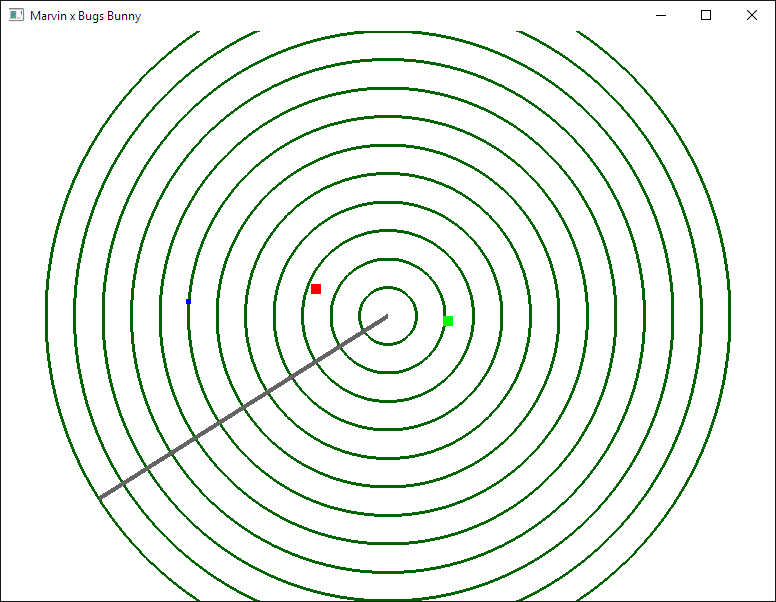
\includegraphics[width=.5\textwidth]{img/cap5_ex20.png}}
    \caption{Sonar}
    \label{fig:cap04_ex1}
  \end{figure}
\end{enumerate}

\section*{Soluções}

\subsection*{Exercício \ref{ex:cap05_ex1} }

\lstinputlisting[caption=Simulador de inundação, style=customc, label=lst:cap5_ex1]{src/ex18_geiser.cpp}

\subsection*{Exercício \ref{ex:cap05_ex2} }

\lstinputlisting[caption=Lua em órbita espiral, style=customc, label=lst:cap5_ex2]{src/ex19_luaespiral.cpp}

\subsection*{Exercício \ref{ex:cap05_ex3} }

\lstinputlisting[caption=Sonar, style=customc, label=lst:cap5_ex2]{src/ex20_sonar.cpp}


% \chapter{First Edited Book Sample Chapter Title}
% \chapterauthors{G. Alvarez and R. K. Watts
% \chapteraffil{Carnegie Mellon University, Pittsburgh, Pennsylvania}
% }

% \section{Here is a normal section}
% Here is some text.


% \chapter{Second Edited Book Sample Chapter Title}
% \chapterauthors{George Smeal, Ph.D.\affilmark{1}, Sally Smith,
% M.D.\affilmark{2} and Stanley Kubrick\affilmark{1}
% \chapteraffil{\affilmark{1}AT\&T Bell Laboratories
% Murray Hill, New Jersey\\
% \affilmark{2}Harvard Medical School,
% Boston, Massachusetts}
% }

% \section{Sample Section}
% Here is some sample text.

% \newpage

% \section{Example, Figure and Tables}
% \vskip6pt
% \begin{example}[Optional Example Name]
% Use Black's law [Equation (6.3)] to estimate the reduction in useful product
% life if a metal line is initially run at 55$^\circ$C at a maximum line
% current density.
% \end{example}




% \begin{figure}[ht]
% illustration here
% %\centerline{\includegraphics[width=.5\textwidth]{filename}}
% \caption{Short figure caption.}
% \end{figure}

% \begin{figure}[ht]
% \vskip2pt
% \caption{Oscillograph for  memory address access operations,
% showing 500 ps
% address access time and superimposed signals
% of address access in 1 kbit
% memory plane.}
% \end{figure}

% \begin{table}[ht]
% \caption{Small Table}
% \centering
% \begin{tabular}{cccc}
% \hline
% one&two&three&four\\
% \hline
% C&D&E&F\\
% \hline
% \end{tabular}
% \end{table}



% \begin{table}[ht]
% \caption{Effects of the two types of $\alpha\beta\sum^A_B$ scaling proposed by Dennard \newline
% and
% co-workers$^{a,b}$}
% \begin{tabular*}{\textwidth}{@{\extracolsep{\fill}}lcc}
% \hline
% Parameter& $\kappa$ Scaling & $\kappa$, $\lambda$ Scaling\cr
% \hline
% Dimension&$\kappa^{-1}$&$\lambda^{-1}$\cr
% Voltage&$\kappa^{-1}$&$\kappa^{-1}$\cr
% Currant&$\kappa^{-1}$&$\lambda/\kappa^{2}$\cr
% Dopant Concentration&$\kappa$&$\lambda^2/\kappa$\cr
% \hline
% \end{tabular*}
% \begin{tablenotes}
% $^a$Refs.~19 and 20.

% $^b\kappa, \lambda>1$.
% \end{tablenotes}
% \end{table}

% \subsection{Side by Side Tables and Figures}

% \begin{figure}[ht]
% \sidebyside{
% Space for figure...
% \caption{This caption will go on the left side of
% the page. It is the initial caption of two side-by-side captions.}
% }
% {
% Space for second figure...
% \caption{This caption will go on the right side of
% the page. It is the second of two side-by-side captions.}
% }
% \end{figure}


% The command \verb+\sidebyside{}{}+ works similarly for tables:

%  \begin{table}[ht]
%  \sidebyside{
% \caption{Table Caption} 
% \begin{tabular}{cccc}
% one&two&three&four\\
% a &little&sample&table
% \end{tabular}
% }
%  {
% \caption{Table Caption}
% \begin{tabular}{cccc}
% A&B&C&D\\
% a &second little& sample&table
% \end{tabular}
% }
%  \end{table}


% When using \verb+\sidebyside+, one must
% use the cross referencing command \verb+\label{}+ after and  {\it outside} 
%  of \verb+\caption{}+:

% \begin{verbatim}
%  \begin{table} 
%  \sidebyside{\caption{Table Caption}\label{tab1}
%  first table}
%  {\caption{Table Caption}\label{tab2} second table}
%  \end{table}
% \end{verbatim}
%  or,
% \begin{verbatim}
%  \begin{figure} 
%  \sidebyside{\vskip<dimen>\caption{fig caption}\label{fig1}}
%  {\vskip<dimen>\caption{fig caption}\label{fig2}}
%  \end{figure}
% \end{verbatim}



% \section{Algorithm}
% This is a sample algorithm.

% \begin{algorithm}
% {\bf state\_transition algorithm} $\{$
% \        for each neuron $j\in\{0,1,\ldots,M-1\}$
% \        $\{$   
% \            calculate the weighted sum $S_j$ using Eq. (6);
% \            if ($S_j>t_j$)
% \                    $\{$turn ON neuron; $Y_1=+1\}$   
% \            else if ($S_j<t_j$)
% \                    $\{$turn OFF neuron; $Y_1=-1\}$   
% \            else
% \                    $\{$no change in neuron state; $y_j$ remains %
% unchanged;$\}$ 
% \        $\}$   
% $\}$   
% \end{algorithm}

% Here is some normal text.
% Here is some normal text.
% Here is some normal text.
% Here is some normal text.
% Here is some normal text.
% Here is some normal text.
% Here is some normal text.
% Here is some normal text.
% Here is some normal text.
% Here is some normal text.
% Here is some normal text.
% Here is some normal text.
% Here is some normal text.
% Here is some normal text.


% \begin{quote}
% This is a sample of extract or quotation.
% This is a sample of extract or quotation.
% This is a sample of extract or quotation.
% \end{quote}

% \begin{enumerate}
% \item
% This is the first item in the numbered list.

% \item
% This is the second item in the numbered list.
% This is the second item in the numbered list.
% This is the second item in the numbered list.
% \end{enumerate}

% \begin{itemize}
% \item
% This is the first item in the itemized list.

% \item
% This is the first item in the itemized list.
% This is the first item in the itemized list.
% This is the first item in the itemized list.
% \end{itemize}

% \begin{itemize}
% \item[]
% This is the first item in the itemized list.

% \item[]
% This is the first item in the itemized list.
% This is the first item in the itemized list.
% This is the first item in the itemized list.
% \end{itemize}

% \begin{problems}
% \prob
% For Hooker's data, Problem 1.2, use the Box and Cox and Atkinson procedures to determine a appropriate transformation of PRES
% in the regression of PRES on TEMP. find $\hat\lambda$, $\tilde\lambda$,
% the score test, and the added variable plot for the score. 
% Summarize the results.

% \prob
% The following data were collected in a study of the effect of dissolved sulfur
% on the surface tension of liquid copper (Baes and Killogg, 1953).

% {\centering
% \vskip6pt
% \begin{tabular}{rlcc}
% \hline
% &&\multicolumn2c{$Y$= Decrease in Surface Tension}\\
% \multicolumn2c{$x$ = Weight \% sulfur}
% &\multicolumn2c{(dynes/cm), two Replicates}\\
% \hline
% 0.&034&301&316\\
% 0.&093&430&422\\
% 0.&30&593&586\\
% \hline
% \end{tabular}
% \vskip6pt
% }


% \subprob
% Find the transformations of $X$ and $Y$ sot that in the transformed scale 
% the regression is linear.

% \subprob
% Assuming that $X$ is transformed to $\ln(X)$, which choice of $Y$ gives 
% better results,
% $Y$ or $\ln(Y)$? (Sclove, 1972).

% \sidebysidesubprob{In the case of $\alpha_1$?}{In the case of $\alpha_2$?}

% \prob
% Examine the Longley data, Problem 3.3, for applicability of assumptions of the
% linear model.

% \sidebysideprob{In the case of $\Gamma_1$?}{In the case of $\Gamma_2$?}

% \end{problems}


% \begin{exercises}
% \exer
% For Hooker's data, Exercise 1.2, use the Box and Cox and Atkinson procedures to determine a appropriate transformation of PRES
% in the regression of PRES on TEMP. find $\hat\lambda$, $\tilde\lambda$,
% the score test, and the added variable plot for the score. 
% Summarize the results.

% \exer
% The following data were collected in a study of the effect of dissolved sulfur
% on the surface tension of liquid copper (Baes and Killogg, 1953).

% {\centering
% \vskip6pt
% \begin{tabular}{rlcc}
% \hline
% &&\multicolumn2c{$Y$= Decrease in Surface Tension}\\
% \multicolumn2c{$x$ = Weight \% sulfur}
% &\multicolumn2c{(dynes/cm), two Replicates}\\
% \hline
% 0.&034&301&316\\
% 0.&093&430&422\\
% 0.&30&593&586\\
% \hline
% \end{tabular}
% \vskip6pt
% }


% \subexer
% Find the transformations of $X$ and $Y$ sot that in the transformed scale 
% the regression is linear.

% \subexer
% Assuming that $X$ is transformed to $\ln(X)$, which choice of $Y$ gives 
% better results,
% $Y$ or $\ln(Y)$? (Sclove, 1972).

% \sidebysidesubexer{In the case of $\Delta_1$?}{In the case of $\Delta_2$?}

% \exer
% Examine the Longley data, Problem 3.3, for applicability of assumptions of the
% linear model.

% \sidebysideexer{In the case of $\Gamma_1$?}{In the case of $\Gamma_2$?}

% \end{exercises}


% \section{Summary}
% This is a summary of this chapter.
% Here are some references: \cite{xkilby}, \cite{xberen}.

% \begin{chapreferences}{5.}
% \bibitem{xkilby}J. S. Kilby,
% ``Invention of the Integrated Circuit,'' {\it IEEE Trans. Electron Devices,}
% {\bf ED-23,} 648 (1976).


% \bibitem{xhamming}R. W. Hamming,
%                  {\it Numerical Methods for Scientists and 
%                  Engineers}, Chapter N-1, McGraw-Hill, 
%                  New York, 1962.

% \bibitem{xHu}J. Lee, K. Mayaram, and C. Hu, ``A Theoretical
%                Study of Gate/Drain Offset in LDD MOSFETs''
%                      {\it IEEE Electron Device Lett.,} {\bf EDL-7}(3). 152 
%                      (1986).

% \bibitem{xberen}A. Berenbaum, 
% B. W. Colbry, D.R. Ditzel, R. D Freeman, and 
% K.J. O'Connor, ``A Pipelined 32b Microprocessor with 13 kb of Cache Memory,''
% {it Int. Solid State Circuit Conf., Dig. Tech. Pap.,} p. 34 (1987).
% \end{chapreferences}


% \chapappendix{This is the Chapter Appendix Title}
% This is an appendix with a title.
% \begin{equation}
% \alpha\beta\Gamma\Delta
% \end{equation}



% \begin{figure}[ht]
% \caption{This is an appendix figure caption.}
% \end{figure}

% \begin{table}[ht]
% \caption{This is an appendix table caption}
% \centering
% \let\hline\savehline
% \begin{tabular}{@{\vrule height 11pt depth 4pt width0pt}|l|p{.65\textwidth}|c}
% \hline
% {\bf Date} & \multicolumn1{c|}{\bf Event} \\
% \hline \hline
% 1867 & Maxwell speculated the existence of electromagnetic waves.\\
% 1887 & Hertz showed the existence of electromagnetic waves. \\
% 1890 & Branly developed technique for detecting radio waves. \\
% 1896 & Marconi demonstrated wireless telegraph. \\
% 1897 & Marconi patented wireless telegraph.  \\
% 1898 & Marconi awarded patent for tuned communication. \\
% 1898 & Wireless telegraphic connection between England and France established. \\
% \hline
% \end{tabular}
% \end{table}


% \chapappendix{}
% This is a Chapter Appendix without a title.

% Here is a math test to show the difference between using Computer Modern
% math fonts and MathTimes math fonts. When MathTimes math fonts are used
% the letters in an equation will match TimesRoman italic in the text.
% ({\it g, i, y, x, P, F, n, f, etc.}) Caligraphic fonts, used for
% $\cal ABC$ below, will stay the same
% in either case.
% \begin{equation}
% g_i(y|f)=\sum_x P(x|F_n)f_i(y|x){\cal ABC}
% \end{equation}
% where $g_i(y|F_n)$ is the function specifying the probability an object will
% display a value $y$ on a dimension $i$ given $F_n$ the observed feature
% structure of all the objects.
% %% ok


% \appendix{This is the Appendix Title}
% \markboth{Short appendix title}{Short appendix title}
% This is an appendix with a title.
% \begin{equation}
% \alpha\beta\Gamma\Delta
% \end{equation}



% \begin{figure}[ht]
% \caption{This is an appendix figure caption.}
% \end{figure}


% \begin{table}[ht]
% \caption{Appendix table caption}
% \centering
% \begin{tabular}{cccc}
% \hline
% Alpha&Beta&Gamma&Delta\\
% \hline
% $\alpha$&$\beta$&$\Gamma$&$\Delta$\\
% \hline
% \end{tabular}
% \end{table}


% \appendix{}
% This is an appendix without a title.

% Here is a math test to show the difference between using Computer Modern
% math fonts and MathTimes math fonts. When MathTimes math fonts are used
% the letters in an equation will match TimesRoman italic in the text.
% ({\it g, i, y, x, P, F, n, f, etc.}) Caligraphic fonts, used for
% $\cal ABC$ below, will stay the same
% in either case.
% \begin{equation}
% g_i(y|f)=\sum_x P(x|F_n)f_i(y|x){\cal ABC}
% \end{equation}
% where $g_i(y|F_n)$ is the function specifying the probability an object will
% display a value $y$ on a dimension $i$ given $F_n$ the observed feature
% structure of all the objects.


% \appendix{Alternate Reference Styles}

% \begin{references}{3.}
% \bibitem{kilby}J. S. Kilby,
% ``Invention of the Integrated Circuit,'' {\it IEEE Trans. Electron Devices,}
% {\bf ED-23,} 648 (1976).

% \bibitem{hamming}R. W. Hamming,
%                  {\it Numerical Methods for Scientists and 
%                  Engineers}, Chapter N-1, McGraw-Hill, 
%                  New York, 1962.

% \bibitem{Hu}J. Lee, K. Mayaram, and C. Hu, ``A Theoretical
%                Study of Gate/Drain Offset in LDD MOSFETs''
%                      {\it IEEE Electron Device Lett.,} {\bf EDL-7}(3). 152 
%                      (1986).

% \bibitem{beren}A. Berenbaum, 
% B. W. Colbry, D.R. Ditzel, R. D Freeman, and 
% K.J. O'Connor, ``A Pipelined 32b Microprocessor with 13 kb of Cache Memory,''
% {it Int. Solid State Circuit Conf., Dig. Tech. Pap.,} p. 34 (1987).
% \end{references}


% \begin{references}{Ham62}
% \bibitem[Kil76]{kilb}J. S. Kilby,
% ``Invention of the Integrated Circuit,'' {\it IEEE Trans. Electron Devices,}
% {\bf ED-23,} 648 (1976).

% \bibitem[Ham62]{hamm}R. W. Hamming,
%                  {\it Numerical Methods for Scientists and 
%                  Engineers}, Chapter N-1, McGraw-Hill, 
%                  New York, 1962.

% \bibitem[Hu86]{lee}J. Lee, K. Mayaram, and C. Hu, ``A Theoretical
%                Study of Gate/Drain Offset in LDD MOSFETs''
%                      {\it IEEE Electron Device Lett.,} {\bf EDL-7}(3). 152 
%                      (1986).

% \bibitem[Ber87]{berm}A. Berenbaum, 
% B. W. Colbry, D.R. Ditzel, R. D Freeman, and 
% K.J. O'Connor, ``A Pipelined 32b Microprocessor with 13 kb of Cache Memory,''
% {it Int. Solid State Circuit Conf., Dig. Tech. Pap.,} p. 34 (1987).

% \end{references}



%%%%%%%%%%%%%%%
%%  The default LaTeX Index
%%  Don't need to add any commands before \begin{document}
\printindex

%%%% Making an index
%% 
%% 1. Make index entries, don't leave any spaces so that they
%% will be sorted correctly.
%% 
%% \index{term}
%% \index{term!subterm}
%% \index{term!subterm!subsubterm}
%% 
%% 2. Run LaTeX several times to produce <filename>.idx
%% 
%% 3. On command line, type  makeindx <filename> which
%% will produce <filename>.ind 
%% 
%% 4. Type \printindex to make the index appear in your book.
%% 
%% 5. If you would like to edit <filename>.ind 
%% you may do so. See docs.pdf for more information.
%% 
%%%%%%%%%%%%%%%%%%%%%%%%%%%%%%

%%%%%%%%%%%%%% Making Multiple Indices %%%%%%%%%%%%%%%%
%% 1. 
%% \usepackage{multind}
%% \makeindex{book}
%% \makeindex{authors}
%% \begin{document}
%% 
%% 2.
%% % add index terms to your book, ie,
%% \index{book}{A term to go to the topic index}
%% \index{authors}{Put this author in the author index}
%% 
%% \index{book}{Cows}
%% \index{book}{Cows!Jersey}
%% \index{book}{Cows!Jersey!Brown}
%% 
%% \index{author}{Douglas Adams}
%% \index{author}{Boethius}
%% \index{author}{Mark Twain}
%% 
%% 3. On command line type 
%% makeindex topic 
%% makeindex authors
%% 
%% 4.
%% this is a Wiley command to make the indices print:
%% \multiprintindex{book}{Topic index}
%% \multiprintindex{authors}{Author index}

\end{document}

